\documentclass[11pt]{aghdpl}
% \documentclass[en,11pt]{aghdpl}  % praca w języku angielskim

% Lista wszystkich języków stanowiących języki pozycji bibliograficznych użytych w pracy.
% (Zgodnie z zasadami tworzenia bibliografii każda pozycja powinna zostać utworzona zgodnie z zasadami języka, w którym dana publikacja została napisana.)
\usepackage[english,polish]{babel}

% Użyj polskiego łamania wyrazów (zamiast domyślnego angielskiego).
\usepackage{polski}

\usepackage[utf8]{inputenc}

% dodatkowe pakiety

\usepackage{mathtools}
\usepackage{amsfonts}
\usepackage{amsmath}
\usepackage{amsthm}

% --- < bibliografia > ---

\usepackage[
style=numeric,
sorting=none,
%
% Zastosuj styl wpisu bibliograficznego właściwy językowi publikacji.
language=autobib,
autolang=other,
% Zapisuj datę dostępu do strony WWW w formacie RRRR-MM-DD.
urldate=iso8601,
% Nie dodawaj numerów stron, na których występuje cytowanie.
backref=false,
% Podawaj ISBN.
isbn=true,
% Nie podawaj URL-i, o ile nie jest to konieczne.
url=false,
%
% Ustawienia związane z polskimi normami dla bibliografii.
maxbibnames=3,
% Jeżeli używamy BibTeXa:
backend=bibtex
]{biblatex}

\usepackage{csquotes}
% Ponieważ `csquotes` nie posiada polskiego stylu, można skorzystać z mocno zbliżonego stylu chorwackiego.
\DeclareQuoteAlias{croatian}{polish}

\addbibresource{bibliografia.bib}

% Nie wyświetlaj wybranych pól.
%\AtEveryBibitem{\clearfield{note}}


% ------------------------
% --- < listingi > ---

% Użyj czcionki kroju Courier.
\usepackage{courier}

\usepackage{listings}
\lstloadlanguages{TeX}

\lstset{
        literate={ą}{{\k{a}}}1
           {ć}{{\'c}}1
           {ę}{{\k{e}}}1
           {ó}{{\'o}}1
           {ń}{{\'n}}1
           {ł}{{\l{}}}1
           {ś}{{\'s}}1
           {ź}{{\'z}}1
           {ż}{{\.z}}1
           {Ą}{{\k{A}}}1
           {Ć}{{\'C}}1
           {Ę}{{\k{E}}}1
           {Ó}{{\'O}}1
           {Ń}{{\'N}}1
           {Ł}{{\L{}}}1
           {Ś}{{\'S}}1
           {Ź}{{\'Z}}1
           {Ż}{{\.Z}}1,
        basicstyle=\footnotesize\ttfamily,
}

% ------------------------

\AtBeginDocument{
        \renewcommand{\tablename}{Tabela}
        \renewcommand{\figurename}{Rys.}
}

% ------------------------
% --- < tabele > ---

\usepackage{array}
\usepackage{tabularx}
\usepackage{multirow}
\usepackage{booktabs}
\usepackage{makecell}
\usepackage{tikz}
\usepackage{pifont}
\usepackage{subcaption}
\usepackage{graphicx}
\usepackage{float}
\usepackage[flushleft]{threeparttable}

% defines the X column to use m (\parbox[c]) instead of p (`parbox[t]`)
\newcolumntype{C}[1]{>{\hsize=#1\hsize\centering\arraybackslash}X}
\newcommand{\xmark}{\ding{55}}%
\newcommand{\cmark}{\ding{51}}%
\newcolumntype{a}{X}
\newcolumntype{d}{>{\hsize=.4\hsize}X}
%---------------------------------------------------------------------------

\author{Radosław Sajdak}
\author{Mateusz Kozyra}
\shortauthor{R. Sajdak}

%\titlePL{Przygotowanie bardzo długiej i pasjonującej pracy dyplomowej w~systemie~\LaTeX}
%\titleEN{Preparation of a very long and fascinating bachelor or master thesis in \LaTeX}

\titlePL{Opracowanie urządzenia wykrywającego wypadek rowerowy z powiadamianiem GSM}
\titleEN{Development of a bicycle accident detection device with GSM notification}


\shorttitlePL{Opracowanie urządzenia wykrywającego wypadek rowerowy} % skrócona wersja tytułu jeśli jest bardzo długi
\shorttitleEN{Development of a bicycle accident detection device}

\thesistype{Praca dyplomowa inżynierska}
%\thesistype{Master of Science Thesis}

\supervisor{dr inż. Łukasz Krzak}
%\supervisor{Marcin Szpyrka PhD, DSc}

\degreeprogramme{Elektronika i Telekomunikacja}
%\degreeprogramme{Computer Science}

\date{2022}

\department{Katedra Elektroniki}
%\department{Department of Applied Computer Science}

\faculty{Wydział Informatyki, Elektroniki,\protect\\[-1mm] i Telekomunikacji}
%\faculty{Faculty of Electrical Engineering, Automatics, Computer Science and Biomedical Engineering}

\acknowledgements{Serdecznie dziękuję \dots tu ciąg dalszych podziękowań np. dla promotora, żony, sąsiada itp.}


\setlength{\cftsecnumwidth}{10mm}

%---------------------------------------------------------------------------
\setcounter{secnumdepth}{4}
\brokenpenalty=10000\relax


\begin{document}

\begin{titlepage}
        \begin{center}
        \begin{tabular}[t]{|p{6cm}|p{9cm} |}
        \hline
        \begin{minipage}{.3\textwidth}
                \centering
                
\includegraphics[width=30mm]{Graphics/Znak_graficzny_AGH.png}
        \end{minipage} & Akademia Górniczo-Hutnicza\newline im. Stanisława Staszica w Krakowie. \newline Wydział Informatyki, Elektroniki i Telekomunikacji  \\
        \hline
        \multicolumn{2}{|c|}{Sensory w aplikacjach wbudowanych} \\
        \multicolumn{2}{|c|}{ \textbf{SPRAWOZDANIE}} \\
        \multicolumn{2}{|c|}{ Rok I, Systemy wbudowane, Elektronika i Telekomunikacja IIst.} \\
        \hline
        \multicolumn{2}{|c|}{\rule{0pt}{0.5cm}Temat: Moduł z sensorami oparty na procesorze STM32F103, zgodny z wyprowadzeniami Mikrobus\texttrademark\rule[-0.25cm]{0pt}{0.5cm}} \\
        \hline
        \rule{0pt}{0.5cm}Zespół: \newline 1. Mateusz Kozyra \newline 2. Mirosław Wiącek \newline 3. Radosław Sajdak & 
        \rule{0pt}{0.5cm}Oceny indywidualne: \newline 1. \newline 2. \newline 3. \newline \\
        \hline
        Data oddania sprawozdania: & Ocena sprawozdania: \newline \newline\newline \\
        \hline
        Uwagi prowadzącego zajęcia: & Informacje dodatkowe: \rule[-3cm]{0pt}{3cm} \\
        \hline
        \end{tabular}
        \end{center}
\end{titlepage}
% Ponowne zdefiniowanie stylu `plain`, aby usunąć numer strony z pierwszej strony spisu treści i poszczególnych rozdziałów.
\fancypagestyle{plain}
{
        % Usuń nagłówek i stopkę
        \fancyhf{}
        % Usuń linie.
        \renewcommand{\headrulewidth}{0pt}
        \renewcommand{\footrulewidth}{0pt}
}

\setcounter{tocdepth}{2}
\tableofcontents
\clearpage

\chapter{Wstęp}
\label{cha:introduction}
Założeniem projektu, było stworzenie modułu sensora, zgodnego ze standardem mikroBUS\texttrademark. Zespół, korzystając z okazji na zdobycie nowych umiejętności, zdecydował się rozszerzyć założenia projektowe o dwa dodatkowe sensory (co daje łącznie trzy układy pomiarowe na jednej płytce). Układy te, komunikują się z mikroprocesorem STM32F103 znajdującym się na tej samej płyce. W procesorze, dane są przetwarzane, nakładając dodatkową warstwę abstrakcji dla obsługi sensorów. Z płytką, można komunikować się przy użyciu interfejsu UART. Dodatkowym założeniem projektu, było różne podejście do tworzenia oprogramowania, każdego z członków zespołu. Zdecydowano, że jeden będzie tworzyć kod, testując go z mikroprocesorem STM32F4, kolejny bezpośrednio na wykonanej płyce, a ostatni, bez bezpośredniej styczności ze sprzętem. Podejście to, pozwoliło spojrzeć na pojekt z innej perspektywy, jak gdyby zespół był większy i rozproszony. Całe proces tworzenia był kontrolowany przy użyciu platformy Github, pozwalającej na wygodną kontrolę wersji oraz dyskusję nad kolejnymi zmianami w kodzie. \newline
W niniejszym sprawozdaniu, skupiono się przede wszystkim na procesie tworzenia modułu oraz popełnionych błędach, nie pomijając krótkiego wstępu teoretycznego. Całość, zakończona jest wnioskami na temat procesu oraz zdobytych umiejętności.
\section{mikroBUS\texttrademark}
MikroBus\texttrademark jest standardem definiującym układ gniazd oraz wyprowadzeń na płytce, zawierającej układ scalony (np. sensor). Standard opisuje również dokładne wymiary płytki, a także narzuca warstwę nadruków na płytce. Założeniem mikroBUS\texttrademark, jest umożliwienie szybkiego i łatwego rozbudowywania układów na rzecz prototypowania. Dostarczane przez wielu producentów płytki z gotowymi gniazdami, pozwalają w prosty sposób uruchomić dowolny sensor, a następnie stworzyć dla niego oprogramowanie. Tym samym, mikroBUS\texttrademark okazuje się świetną alternatywą dla niestabilnych płytek stykowych. Na rysunku \ref{img:mikrobus_pinout} przedstawiono zdefiniowany w standardzie pinout. \newline
Ze względu na zmienione założenia projektu, stworzona płytka zgadza się ze standardem co do wyprowadzeń i wymiarów, jednak nie posiada naniesionych nadruków. Wynika to wprost z braku miejsca, na płytce. Dodatkowo, kilka sensorów na jednej płytce, również nie jest zgodne ze standardem.

\begin{figure}[H]
    \centering
    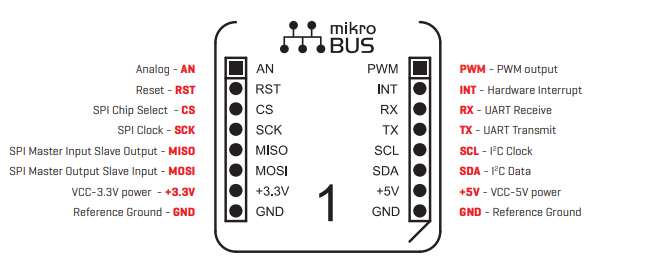
\includegraphics[width=12cm]{Graphics/mikrobus_pinout.png}
    \caption{Specyfikacja wyprowadzeń mikroBUS\texttrademark \cite{mikrobus_specification}}
    \label{img:mikrobus_pinout}
\end{figure}


\section{STM32F103}
Do stworzenia projektu, wybrano procesor STM32F103C8 z rdzeniem ARM\textregistered Cortex\textregistered-M3. Wybór, podyktowany był przede wszystkim dostępnością, ponieważ układ ten, w obudowach LQFP48 znajdował się w prywatnych zasobach zespołu. Obecnie, na rynku dostępne jest niewiele procesorów, a części elektroniczne są drogie. Z tego powodu, zdecydowano się korzystać z tego, co było dostępne. Nie oznacza to jednak, że procesor ten był pod jakimkolwiek względem ograniczający. Najistotniejszymi z jego cech są:
\begin{itemize}
    \item 2 interfejsy I$^2$C
    \item 3 interfejsy USART
    \item 2 interfejsy SPI
    \item Zasilanie 2.0 - 3.6V
    \item Zewnętrzny zegar 4 - 16MHz
    \item 12-bitowe, wielokanałowe przetworniki A/D
\end{itemize}
Układ, programowany jest przy użyciu interfejsu SWD oraz programatora ST-link. Fakt ten, znacząco ułatwił wykonanie działającego układu. Ze względu na przyjęte założenia i wybrane sensory, wybrany procesor bardzo dobrze wpasowywał się w projekt. Dla wykonania oprogramowania, istotne były również dostarczone przez ST biblioteki oraz oprogramowanie STM32CubeMX, wprowadzające wysoki poziom abstrakcji w tworzeniu oprogramowania. Pozwoliło to uniknąć często czasochłonnego, ręcznego pisania do rejestrów procesora, w celu konfiguracji peryferiów. Były również momenty, w których HAL okazał się problemem, co wspomniane zostało w dalszej części sprawozdania.

\section{STS30}

Krótki opis sensora Mirka

\section{BMP280}

Krótki opis sensora Matiego

\section{MQ2}

Krótki opis sensora Matiego

\section{Makefile}
Jak wspomniano we wstępie, jednym z założeń, było tworzenie oprogramowania równolegle, na dwóch różnych procesorach. STM32F1 i STM32F4. Procesory te, należąc do zupełnie różnych rodzin, korzystają z innych bibliotek, a do ich konfiguracji niejednokrotnie wymagane są różne kroki. Z tego powodu, w projekcie wykorzystano program \emph{Make}. Pozwala on, na podstawie pliku konfiguracyjnego \emph{makefile}, zdefiniować sposób kompilacji oraz ścieżki bibliotek wykorzystywanych przez kod. Narzędzie to, jest stosunkowo proste w konfiguracji, a jej przykłady są ogólnodostępne w internecie. Dodatkowym argumentem przemawiającym za jego wykorzystaniem, była chęć jego przetestowania w praktyce.

\section{Github}
Github, to serwis internetowy pozwalający przechowywać projekty z wykorzystaniem systemu kontroli wersji. Korzysta on z systemu Git opublikowanego na licencji GNU GPL 2 (wolne i otwarte oprogramowanie). System ten, jest obecnie wykorzystywany przez wielu programistów, a jego znajomość często wymagana jest przez pracodawców. Github, poza kontrolą wersji, dostarcza wygodne i przejrzyste środowisko w przeglądarce, pozwalające programistom na np. przegląd kodu współpracowników. Fakt ten, został wykorzystany podczas tworzenia projektu. Pozwoliło to nie tylko na poprawienie jakości tworzonego oprogramowania, ale również skonfrontowanie różnych podejść do współpracy nad kodem.
\chapter{Wykonanie projektu}
\label{cha:course}

\section{Projekt płytki}
\subsection{Schemat}
Projekt płytki, naturalnie rozpoczęto od wykonania schematu ideowego. W tym celu przyjęto następujące założenia:
\begin{itemize}
    \item Układ, musi być zasilany zewnętrznie (5v oraz 3.3V)
    \item Wykorzystany zostanie konwerter UART-USB
    \item Układ, będzie można wyłączyć tranzystorem, sterującym przetwornicami
    \item Wykorzystany zostanie zewnętrzny generator
\end{itemize}
Według standardu mikroBUS\texttrademark, płytka zasilana jest przez układ w który jest wpięta. Często jest to zasilanie procesora, na którym tworzone jest oprogramowanie. Ponieważ w opisywanym projekcie, wykorzystany został procesor, oraz trzy sensory (w tym jeden pracujący z napięciem 5V), zdecydowano się na zasilanie zewnętrzne. Miało ono zminimalizować prawdopodobieństwo nieprawidłowej pracy układu. Jednocześnie, czujnik MQ2 pobierając setki mA prądu, mógłby uszkodzić przetwornicę układu w który została wpięta płytka. Najprostszym rozwiązaniem, było wyprowadzenie portu USB i zasilanie z niego układu. Zwrócono uwagę na fakt, że USB w komputerach, nie ma stabilnego napięcia 5V, a często wręcz 4.7-4.8V. Jest to zachowanie zdefiniowane w standardzie USB 2.0 \cite{usb_specification} w rozdziale 7. Z tego powodu , należało wykorzystać regulator napięcia. \newline Wybór tego i wszystkich kolejnych komponentów, podyktowany był w dużej mierze dostępnością na rynku. Kolejnym kryterium, były parametry układu, opisywane w dostarczanych przez producentów dokumentacjach. Jako układ do zasilania sensora MQ2, wykorzystano przetwornicę typu BOOST - MCP1642 o wyjściowym napięciu właśnie 5V. Pozwoliła ona na stabilne zasilenie czujnika. Jej ważną cechą, jest maksymalny prąd na wyjściu, o wartości 800mA. Wysoki prąd jest tutaj niezbędny, ponieważ zasilanie wspomnianego czujnika wymaga nawet 200mA prądu stałego. Do zasilania reszty elementów, wykorzystano regulator LDO  MIC5365 o wyjściowym napięciu 3.3V. Gwarantowany prąd wyjściowy regulatora to 150mA, co jest wartością wystarczającą do zasilenia reszty elementów z zapasem. Całość, z założenia włączana miała być tranzystorem NMOS 2N7002. Bramka tego tranzystora, połączona jest z pinem RESET standardu mikroBUS\texttrademark, pozwalając użytkownikowi wyłączyć układ. W przypadku tego elementu, pojawiły się dwa błędy, wymagające przerobienia gotowej płytki. Problem, szerzej opisano w podrozdziale \ref{sub:mistakes}. \newline
Schemat oraz layout, wykonane zostały w programie KiCad. Opensourcowym oprogramowaniu dla różnych systemów operacyjnych. Program ten, umożliwia podział schematu na bloki, co wykorzystano przenosząc sekcję zasilania do osobnego schematu. Na schemacie \ref{img:power_sch} przedstawiono całą, wspomnianą sekcję. Zasilanie, doprowadzone jest z USB do obu przetwornic. Gdy procesor jest zasilony, a więc działa przetwornica 3.3V, włączona zostaje czerwona dioda LED. Widoczny na schemacie rezystor R10, nie jest uwzględniony w layoucie i został dołożony ręcznie do płytki. Więcej na ten temat, opowiada podrozdział \ref{sub:mistakes}.
\newline Na schemacie, widoczna jest również znacząca ilość kondensatorów. Zostały one dodane do schematu, jako wskazane przez producenta jako konieczne dla poprawnego działania układów. Bardzo istotny jest również rezystor R7, gwarantujący ustalony stan niski po wyłączeniu tranzystora.
\begin{figure}[H]
    \centering
    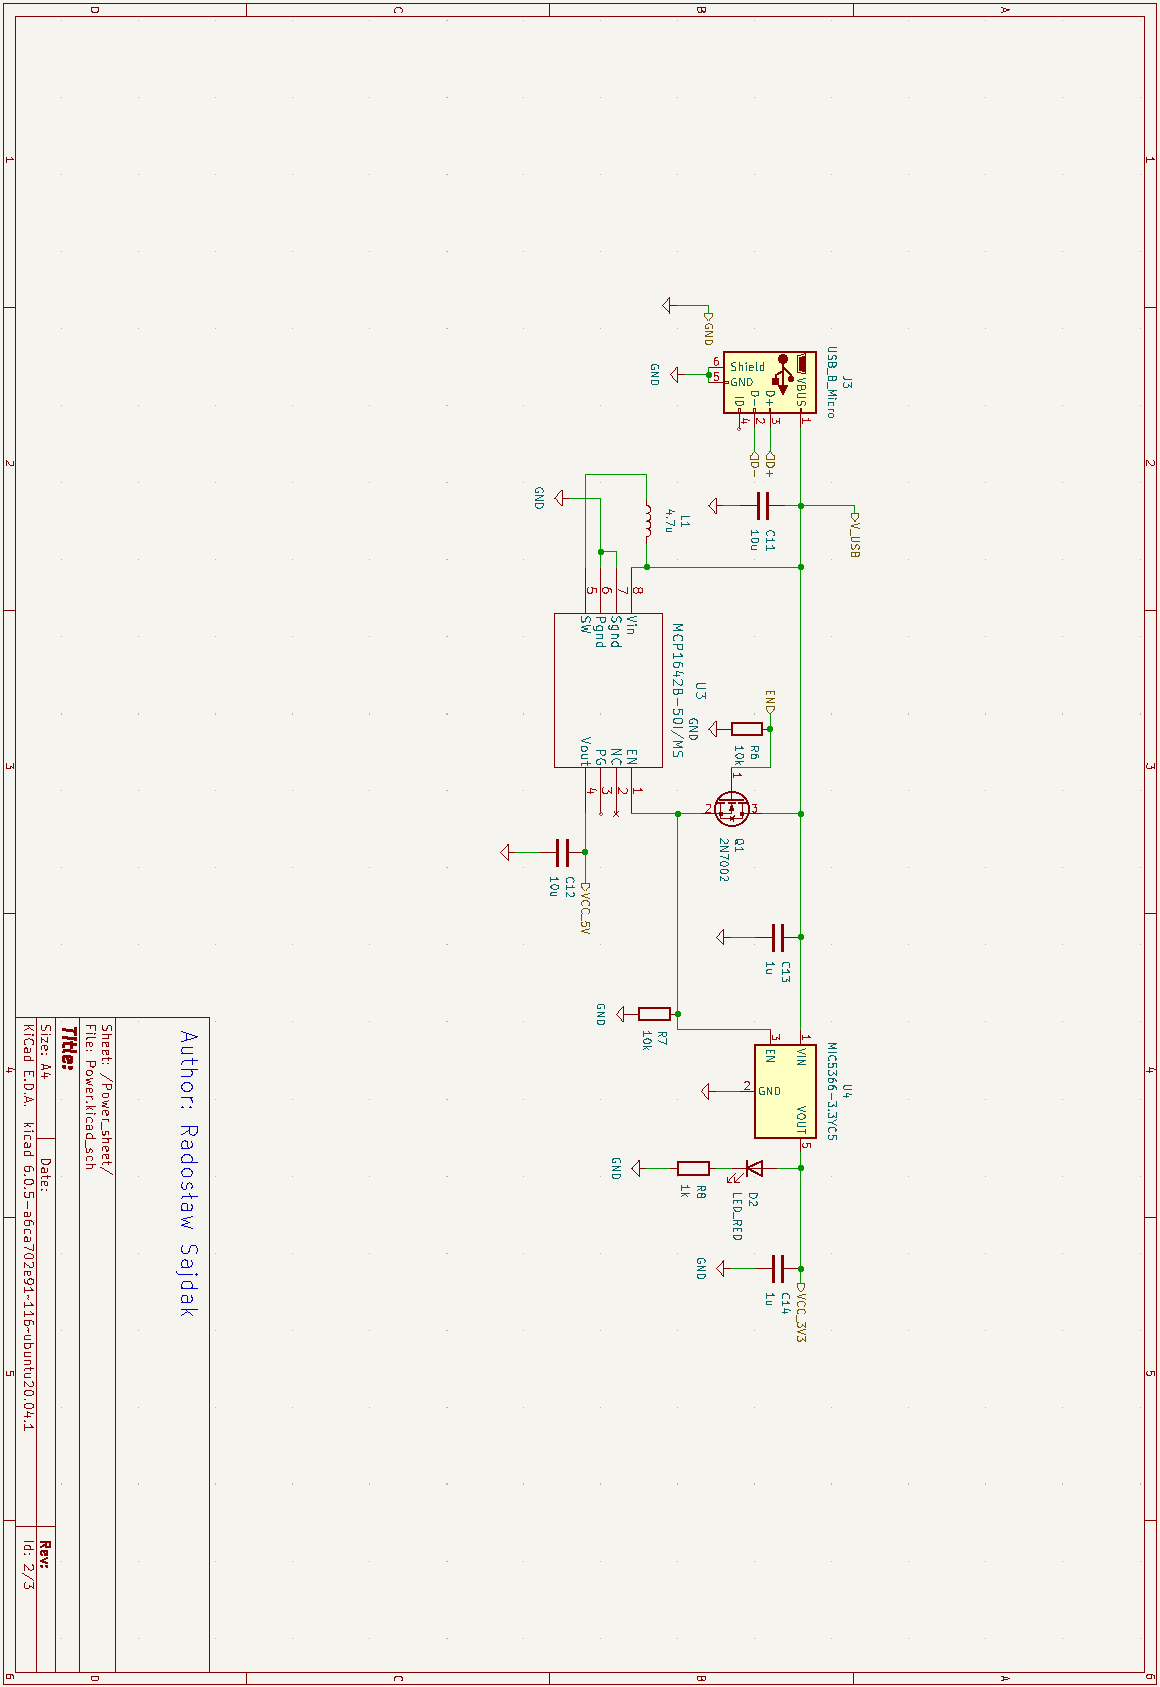
\includegraphics[width=\textwidth, height=\textheight, keepaspectratio]{Graphics/power_sch.png}
    \caption{Schemat części zasilającej moduł}
    \label{img:power_sch}
\end{figure}
Kolejnym blokiem, jest schemat \ref{img:sensors_sch}, zawierający w sobie wszystkie czujniki. Podobnie jak wcześniej, producenci w swoich dokumentacjach zalecają stosowanie kondensatorów, jak najbliżej zasilania układu, dla zapewnienia jego prawidłowego działania. W przypadku sensora działającego z użyciem SPI - BMP280 - zastosowano rezystor pull-down na linii MISO. Dzięki temu, gdy linia nie jest używana, zagwarantowany jest stan niski. Podobnie w przypadku linii NSS. Zastosowanie rezystora podciągającego do zasilania, pozwala zagwarantować, że układ nie będzie aktywny gdy nie jest to pożądane.\newline
Wartym uwagi jest układ czujnika analogowego MQ2. Ze względu na zastosowany procesor, mierzone przetwornikiem napięcie, musi mieścić się w przedziale 0-3.6V. Ponieważ wybrany czujnik działa w zakresie 0-5V, konieczne jest zastosowanie dzielnika napięcia. W tym przypadku, układ rezytorów oraz czujnika, staje się źródłem prądu, który mógłby uszkodzić procesor. Z tego powodu, zastosowano wzmacniacz operacyjny w konfiguracji nieodwracającego wtórnika napięciowego. Wzmacniacz operacyjny, mający bardzo małą rezystancję wyjściową, stanowi w przybliżeniu źródło napięcia równe co do wartości spadkowi napięcia na R11.
\newline
\newline
Ostatnim, a zarazem najistotniejszym, jest schemat \ref{img:main_sch}. Po jego lewej stronie, zaznaczono fragment odpowiadający za konwersję UART-USB. Wykorzystany układ konwertera to CP2102. Układ ten, pozwala obserwować logi mikroprocesora przy użyciu tego samego przewodu, którym zasilamy płytkę. W trakcie tworzenia schematu, rozważano również tylko wyprowadzenie testpointów, pozwalających na podejrzenie logów zewnętrznym konwerterem. Ponieważ jednak planowany jest również inny projekt, wykorzystujący wiele takich konwerterów, zdecydowano się na jego użycie w celach przede wszystkim edukacyjnych i testowych. Głównym zagadnieniem z nim z związanym, było użycie pary różnicowej, wymaganej dla prawidłowegodziałania USB.
\newline
Po prawej stronie schematu \ref{img:main_sch}, widoczny jest blok mikroprocesora STM32F103C8. Zastosowano tutaj zewnętrzny generator o taktowaniu 8MHz, zastępując wewnętrzny zegar mikroprocesora. Istotnym zaganieniem, wymaganym przez mikroprocesor według dokumentacji, jest montaż osobnych kondensatorów o wartości 100n przy każdym z pinów zasilania, możliwie jak najbliżej układu. Dla zapewnienia prawidłowego działania magistrali I$^2$C, dodano rezystory podciągające linie do zasilania. Wszystkie piny posiadają też testpointy, mające ułatwić tworzenie oprogramowania dzięki szybkiemu wykryciu błędów w transmisji, a więc np. w zlutowaniu układu. Dodatkowo, na pinie 8, wyprowadzono LED. Zgodnie z przyjętymi przez zespół założeniami, wskazuje on gotowość układu do pracy, a więc przejście wszystkich kroków inicjalizacyjnych.
\newline
Wartym zaznaczenia jest tutaj fakt nie wyprowadzenia pinów SWDIO oraz SWCLK. Ponieważ są to piny wymagane tylko na etapie tworzenia oprogramowania, podjęto decyzję o ich niewykorzystaniu. Ważną w tym wypadku kwestią, był również brak miejsca na ścieżki, pozwalające na taki zabieg. Niemniej jednak, osoba składająca PCB, bez większych problemów była w stanie wlutować przewody programatora bezpośrednio do pinów mikroprocesora.
\begin{figure}[H]
    \centering
    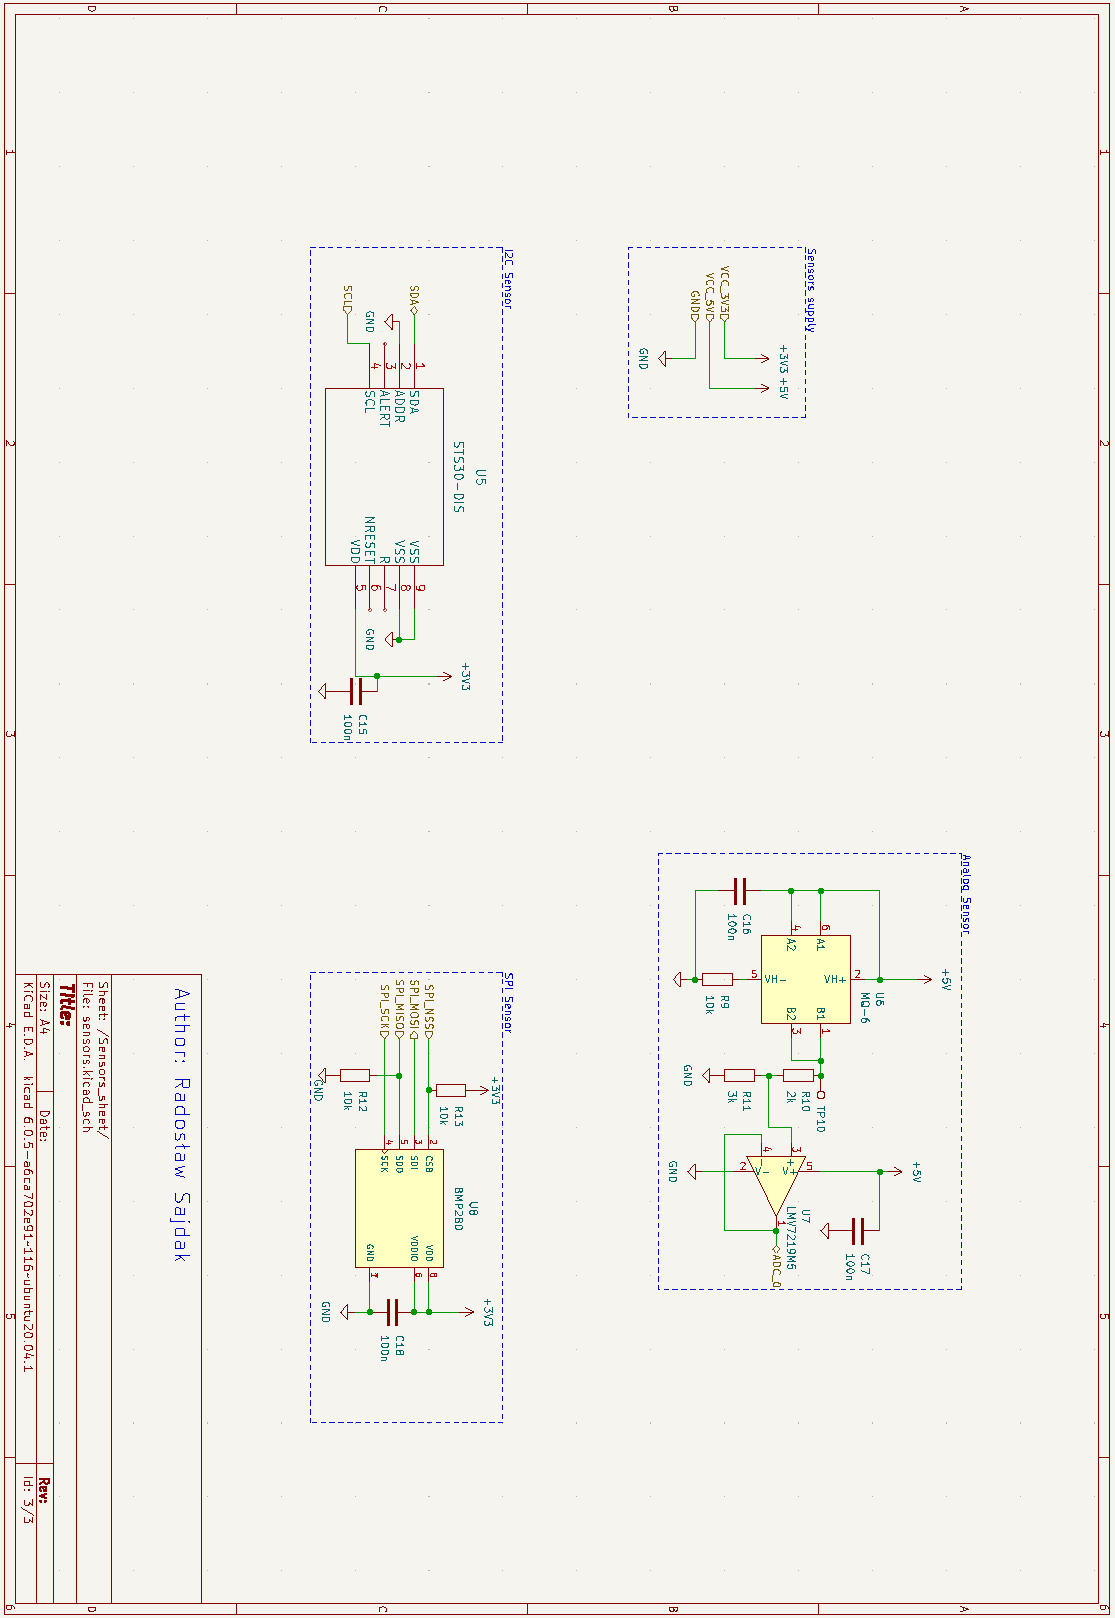
\includegraphics[width=\textwidth, height=\textheight, keepaspectratio]{Graphics/sensors_sch.png}
    \caption{Schemat połączeń czujników}
    \label{img:sensors_sch}
\end{figure}
\begin{figure}[H]
    \centering
    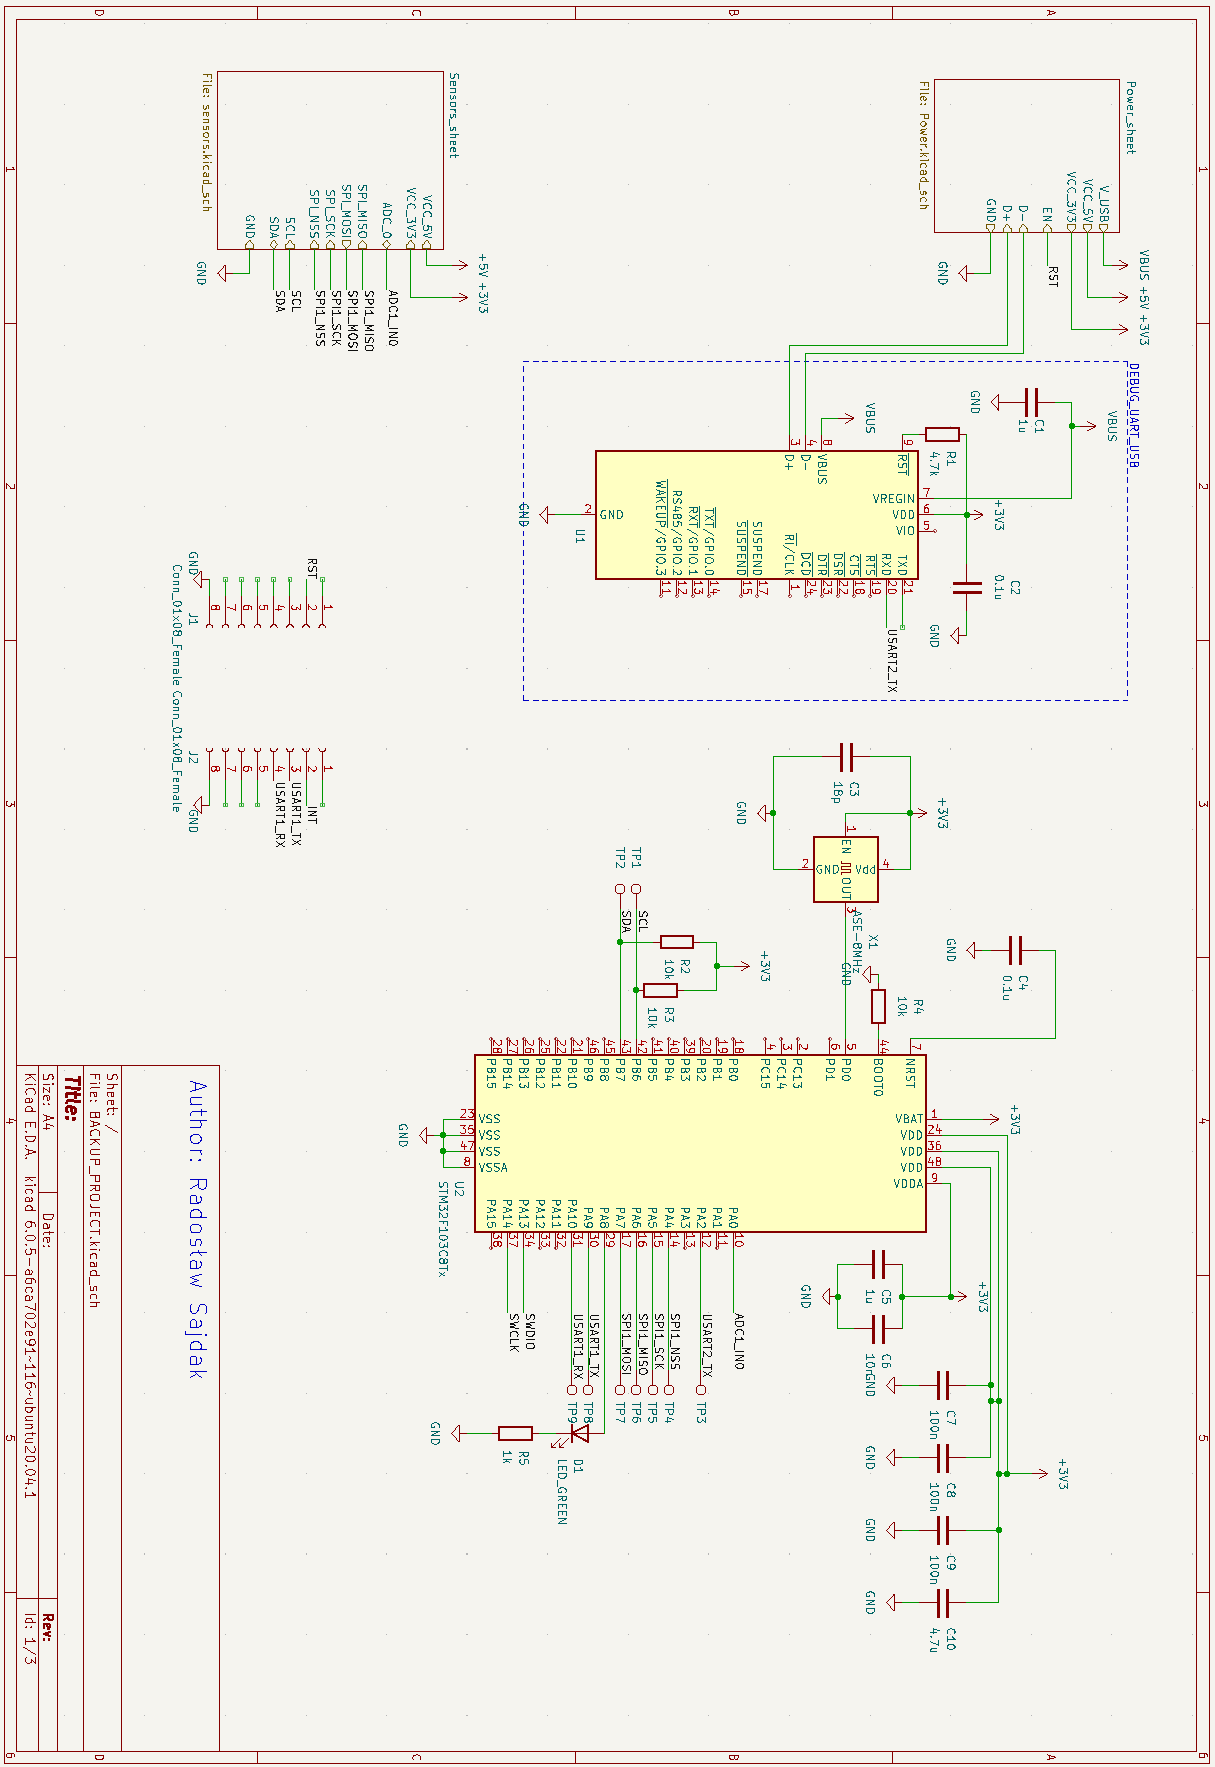
\includegraphics[width=\textwidth, height=\textheight, keepaspectratio]{Graphics/main_sch.png}
    \caption{Schemat połączeń konwertera UART-USB oraz mikroprocesora}
    \label{img:main_sch}
\end{figure}
\subsection{Layout}
\textbf{Pokazać warstwy elektryczne. Zdjęcia wydrukowanych płytek. Jakie problemy się pojawiły (1 raz z Kicadem, więc np. okazało się, że domyślnie ścieżki ma całkiem szerokie. Podobnie viasy). Brak miejsca na wyprowadzenia SWD}

\subsection{Popełnione błędy oraz wykonane przeróbki}
\label{sub:mistakes}
\begin{itemize}
    \item Pokazać odcięcie LDO konwertera
    \item Bramka wisząca w powietrzu
    \item Zła przetwornica 5V (Vin > Vout)
    \item Źle wsadzony mosfet. Pokazać możliwe przeróbki (OPAMP, rezystory, zdjęcia z prób i cięć).
    \item Bypass przetwornicy
    \item Ręczne lutowanie SWD do procka
\end{itemize}


\section{Oprogramowanie}
\subsection{Biblioteki peryferiów}
Na etapie planowania projektów, podjęto decyzję o samodzielnym stworzeniu bibliotek do każdego z czujników. Takie podejście, narzuciło konieczność ujednolicenia sposobu tworzenia kodu. Zdecydowano, że każda biblioteka, będzie korzystać z nakładki na funkcje HALa. Pozwoliło to wprowadzić obsługę błędów na wszystkich poziomach oprogramowania. Kod, tworzony był w sposób możliwie uniwersalny. Dzięki temu, płytka może być łatwo rozbudowana o kolejne czujniki, przy jednocześnie niewielkich zmianach w kodzie programu. Poniżej, krótko omówiono oprogramowanie każdego z czujników, oraz związane z nim biblioteki. Dla zachowania porządku, zdecydowano się rozdzielić w projekcie sterowniki dostarczane przez ST, pliki nagłówkowe oraz stworzone biblioteki. Zastosowanie opisanego w rozdziale \ref{cha:introduction} makefile, pozwoliło w łatwy sposób zdefiniować ścieżki dla kompilatora.
\newline
\textbf{BMP280}
\newline
Pierwszy z czujników, jest czujnikiem komunikującym się z mikroprocesorem z wykorzystaniem SPI (Serial Peripheral Interface). Pozwala on na wykonywanie pomiarów temperatury oraz ciśnienia. Stworzona biblioteka \textit{,,spi.c''} pozwala w łatwy sposób zainicjalizować peryferium w zdefiniowany sposób, odpowiedni dla stworzonej płytki. Osobna funkcja inicjalizująca piny SS (Slave Select) umożliwia szybkie dodanie kolejnych czujników działających z użyciem SPI. Wymaga to jedynie zainicjalizowania pinu. Dwie kolejne funkcje, odpowiadają za kolejno wysyłanie i odczytywanie danych przy użyciu SPI. Interesującym kierunkiem rozbudowy biblioteki, byłaby możliwość rejestracji pinów SS, co zdjęłoby z użytkownika konieczność samodzielnej kontroli nad używanym interfejsem oraz pinami. W przypadku tej wersji płytki, nie było to jednak konieczne. Biblioteka \textit{,,bmp280.c''} korzystająca z \textit{,,spi.c''}, odpowiada za podstawową obsługę czujnika BMP280. Poza podstawowymi możliwościami konfiguracji zgodnie z dokumentacją producenta, wykonuje wszelkie obliczenia, zdejmując z użytkownika konieczność przeliczenia danych z rejestrów.
\newline
\newline
\textbf{STS3x-DIS}
\newline
Kolejny z czujników to czujnik temperatury. Od poprzednika, różni się większą złożonością i lepszą precyzją. Do komunikacji, wykorzystuje magistralę I$^2$C. Stworzona do jego obsługi biblioteka, pozwala zmieniać jego konfigurację przy użyciu czytelnych stałych. Zapewnia nie tylko obsługę rejestrów czujnika, ale również kontrolę CRC otrzymywanych danych. Dzięki temu, użytkownik może być pewien otrzymywanych wartości.
\newline
\newline
\textbf{MQ-2}
\newline
Ostatni z czujników, to analogowy czujnik gazów. Stworzona do obsługi konwertera A/D inicjalizuje wybrane ADC mikoprocesora oraz konkretny kanał, według wartości odpowiednich dla stworzonej płytki. Posiada również funkcję pobrania próbki wybranego konwertera. Sama biblioteka obsługująca MQ-2, poza inicjalizacją i kalibracją sensora, pozwala użytkownikowi na pobranie przetworzonych lub surowych danych z czujnika, dla wybranego gazu. Dodatkową funkcją, jest możliwość ustawienia alarmu dla wybranego gazu, na zdefiniowany przez użytkownika próg. Przekroczenie wybranej wartości wyzwoli alarm oraz wysteruje pin INT standardu mikroBUS\texttrademark. Aby umożliwić swobodne tworzenie funkcji przerwań czasowych w dowolnej ilości, stworzona została biblioteka \textit{,,timers.c''}. Przy użyciu jednokierunkowej, dynamicznej listy stuktur oraz mechanizmu SysTick (przerwania wyzwalanego co 1ms) użytkownik może dodawać własne funkcje o predefiniowanym typie, a następnie wywołać je po upływie określonego czasu. Dodatkowa flaga, pozwala włączyć okresowe wyzwalanie danej funkcji. Zaletą tego podejścia jest przede wszystkim ,,nieograniczona'' liczba liczników, jednak niepoprawne wykorzystanie biblioteki (np. funkcje o długim czasie wykonywania), może prowadzić do utraty precyzji liczników.
\newline
\newline
\textbf{CP2102}
\newline
Na potrzeby obsługi konwertera UART-USB, służącego do debugu kodu, stworzona została również prosta biblioteka do obsługi UARTu. Zawiera ona konfigurację peryferium oraz funkcję działającą jak printf, która zamiast na wyjście standardowe, kieruje dane na konkretny UART. W podobny sposób działa biblioteka obsługująca UART do komunikacji użytkownika z mikroprocesorem, wspomniana w podrozdziale \ref{sub:api}. Zostały one rozdzielone ze względu na zachowanie czystości w kodzie.
\subsection{API}
\label{sub:api}
Najważniejszym elementem projektu, spinającym wszystko w jedną całość, jest stworzone API (ang. Application Programming Interface). Pozwala ono użytkownikowi na komunikację z czujikami, przy użyciu interfejsu UART. Zdecydowano, że dla uproszczenia komunikacji, układ będzie zachowywać się podobnie do dostępnych na rynków modemów, wykorzystując komendy z przedrostkiem \textit{,,AT+''}. Diagram \ref{img:api_diagram} przedstawia schemat działania API. Zostało ono zrealizowane przy użyciu stałych tablic struktur, zawierających komendę oraz związany z nią callback, czyli wywołanie odpowiedniej funkcji bibliotek sensora. Dla ułatwienia obsługi oraz lepszej czytelności kodu, każdy z czujników posiada własną tablicę wywołań. Tym samym, działanie całego API, to tak naprawdę jedna pętla, wywoływana po wykryciu przez UART komendy \textit{,,AT+''}. Wyszukuje ona komendę na odpowiedniej liście, a następnie wywołuje związaną z nią funkcję. Takie podejście, pozwala w bardzo łatwy sposób rozbudowywać kod w przypadku chęci wykorzystania kolejnych czujników. Jedyne wymagane zmiany, to dodanie kolejnej listy zawierającej komendy oraz powiązane callbacki. Zgodnie z diagramem \ref{img:api_diagram}, w przypadku nierozpoznania komendy \textit{AT} układ zwraca użytkownikowi informację \textit{UNKNOWN} (ang. nieznany). \textbf{Kolejne komendy, rozpoznawane są przez znak kończący linię \textbackslash r}. W przypadku nierozpoznanych danych, przesłanych do mikroprocesora, zwrócona zostanie informacja \textit{ERROR} (ang. błąd).

\begin{figure}[H]
    \centering
    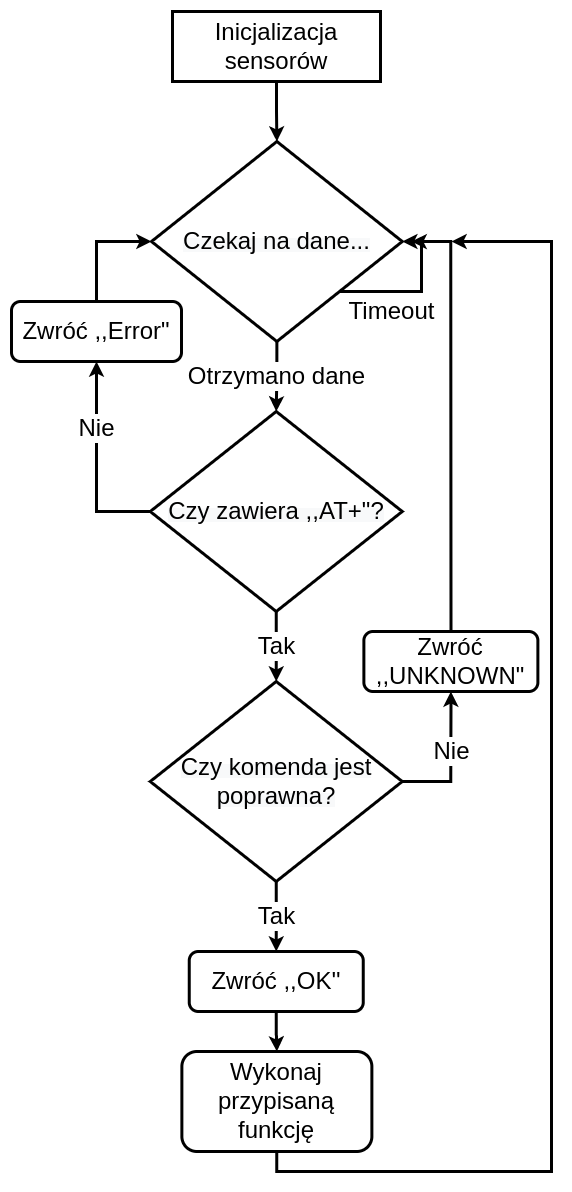
\includegraphics[width=\textwidth, height=\textheight, keepaspectratio]{Graphics/API_Sensors.png}
    \caption{Diagram działania API}
    \label{img:api_diagram}
\end{figure}

\subsection{Lista dostępnych funkcji}
\textbf{Ogólne}\newline
   ,,AT+BMP\textbackslash r'' - Wybiera czujnik BMP280\newline
   ,,AT+STS\textbackslash r'' - Wybiera czujnik STS3x-DIS\newline
   ,,AT+MQ\textbackslash r'' - Wybiera czujnik MQ-2\newline
   ,,AT+BACK\textbackslash r'' - Powrót do menu wyboru czujników\newline

\textbf{BMP280}\newline
   ,,AT+GETDATA\textbackslash r'' - odczytuje próbkę temperatury

\textbf{MQ-2}\newline
   ,,AT+GETDATA\textbackslash r'' - odczytuje stężenie wybranego wcześniej gazu

\textbf{STS3x-DIS}\newline
   ,,AT+GETDATA\textbackslash r'' - Odczytuje próbkę temperatury\newline
   ,,AT+SETREPL\textbackslash r'' - Ustawia dokładność na niską \newline
   ,,AT+SETREPM\textbackslash r'' - Ustawia dokładność na średnią\newline
   ,,AT+SETREPH\textbackslash r'' - Ustawia dokładność na wysoką\newline
   ,,AT+SETHEATON\textbackslash r'' - Włącza wewnętrzną grzałkę\newline
   ,,AT+SETHEATOFF\textbackslash r'' - Wyłącza wewnętrzną grzałkę\newline
   ,,AT+SRESET\textbackslash r'' - Programowy reset czujnika\newline
   ,,AT+BACK\textbackslash r'' - Powrót do menu wyboru czujników\newline

\subsection{System kontroli wersji}
IMHO spoko też napisać, o tym, że korzystaliśmy z tego gita mocno, dbaliśmy o porządek, robiliśmy review itp. To jednak zjadło kupę czasu.

\chapter{Prezentacja działania}
\label{cha:presentation}
Na potrzeby prezentacji działania urządzenia, stworzono przedstawiony na rysunku \ref{img:test_diagram} układ. Układ PC oraz konwertera UART-USB podłączonego do USB0, symulował mikroprocesor z kodem użytkownika. Pozwoliło to na dwukierunkowe przetestowanie działania API oraz samych sensorów. Dodatkowo, dzięki obecnemu na płytce konwerterowi CP2102, przy użyciu USB1 obserwowano tzw. logi programu. W głównej mierze dawały one informację na temat tego, czy dane zostały poprawnie odebrane. Jest to jednak pole do łatwej rozbudowy, ponieważ obecna struktura kodu pozwala wysyłać informacje nt. przebiegu dowolnych funkcji.

\begin{figure}[H]
    \centering
    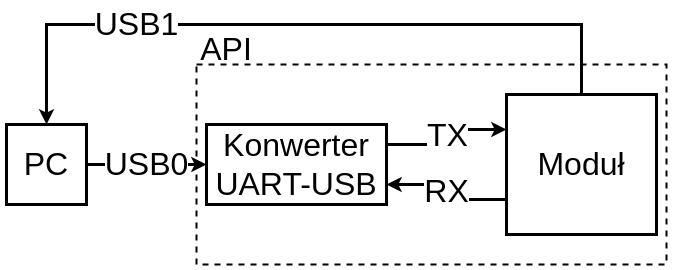
\includegraphics[width=\textwidth, height=\textheight, keepaspectratio]{Graphics/test_sch.png}
    \caption{Diagram aplikacji testowej}
    \label{img:test_diagram}
\end{figure}

Po podłączeniu komponentów zgodnie z powyższym schematem, przy użyciu monitora portu szeregowego Cutecom, wykonano sekwencję komend testujących działanie API. Uporządkowany zapis z monitora, przedstawia obrazek \ref{img:cutecom}. Sekwencję rozpocząto od wyboru czujnika BMP280. Komendy 1-3, opisują prawidłową komunikację z czujnikiem oraz pobranie temperatury. Należy zaznaczyć, że liczba zwracana jest jako 4 bajty danych w formacie fixed point. W celu ich interpretacji, należałoby więc otrzymaną wartość podzielić przez tysiąc. Otrzymana wtedy temperatura, wynosi wówczas 28,631 stopni celcjusza. Czwarta komenda, to przykład wywołanej w niepoprawnym miejscu komendy AT. Ponieważ \textit{,,AT+STS''} nie znajduje się na liście komend sensora BMP280, urządzenie zwróciło informację \textit{UNKNOWN}. Aby wybrany sensor został przełączony poprawnie, należy postępować zgodnie z krokami 5-7. Komenda numer 8, to przykład wykorzystania nieistniejącej komendy AT. Kolejna, \textit{,,WRONGMSG''} to przykład zupełnie niepoprawnych danych. Widać, że układ zgodnie z oczekiwaniami zwrócił wiadomość \textit{ERROR}. Komendą numer 10, pobrano odczyt temperatury z czujnika STS3x-DIS. Wynosi on 37,968 stopni celcjusza. Należy zauważyć, że jest on o około 9 stopni wyższy niż w przypadku odczytu z BMP280. Wynika to  najprawdopodobniej z jego umiejscowienia na płytce, ponieważ znajduje się on nad główną linią zasilania i przetwornicą 5V które w trakcie pracy emitują ciepło, doskonale przenoszone przez miedź na płytce. Wiadomości 11-15 pokazują działającą poprawnie możliwość wpływania na ustawienia czujnika. Uruchomiona wewnętrzna grzałka podniosła temperaturę względem zmierzonej wcześniej, a jej wyłączenie spowodowało spadek mierzonej wartości. W przypadku czujnika MQ-2, komendami 16-19 pobrano aktualną wartość napięcia na pinie związanym z przetwornikiem A/C.\newline
Należy również zwrócić uwagę na dokładność zwracanych temperatur. Rozdzielczość obu czujników to 0,01 stopnia, jednak na podstawie wzorów dostarczanych przez producentów wyliczana jest wartość ,,dokładniejsza''. Aby nie zakłamywać odczytów z czujników, zdecydowano o przekazaniu użytkownikowy wartości odczytanych. Po jego stronie jest więc podjęcie decyzji sposobie zaokrąglania odczytanej wartości oraz uwzględnienie dokładności, wynoszącej $\pm$ 0,2 stopnie. Stworzono również skrypt który przez 5 minut odpytywał naprzemiennie czujnik BMP280 oraz STS3x o temperaturę w celu porównania ich stabilności. Rysunek \ref{img:wykresik} przedstawia zapis tego pomiaru. Około drugiej minuty, do czujników przyłożono palec mający na celu podnieść temperaturę mierzoną. Należy zaznaczyć, że od pomiarów odjęto wartość 8 stopni aby lepiej pokazać zmiany w obu czujnikach. Można zauważyć, że pomiary z czujnika BMP280 są bardziej stabilne, co wynika z obecności filtru IIR. Z wykresu można również stwierdzić, że palec zdecydowanie lepiej pokrywał czujnik BMP280, co przełożyło się na wyższą maksymalną temperaturę.

\begin{figure}[H]
    \centering
    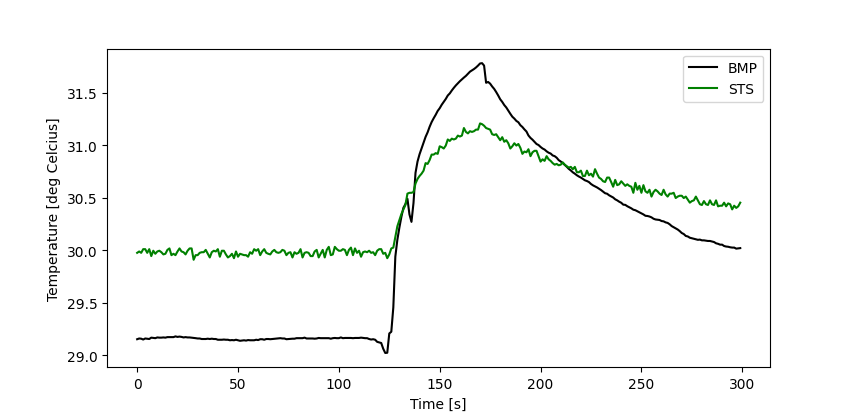
\includegraphics[width=\textwidth, height=\textheight, keepaspectratio]{../Test/Figure_1.png}
    \caption{Zapis pomiaru temperatury}
    \label{img:wykresik}
\end{figure}

\begin{figure}[H]
    \centering
    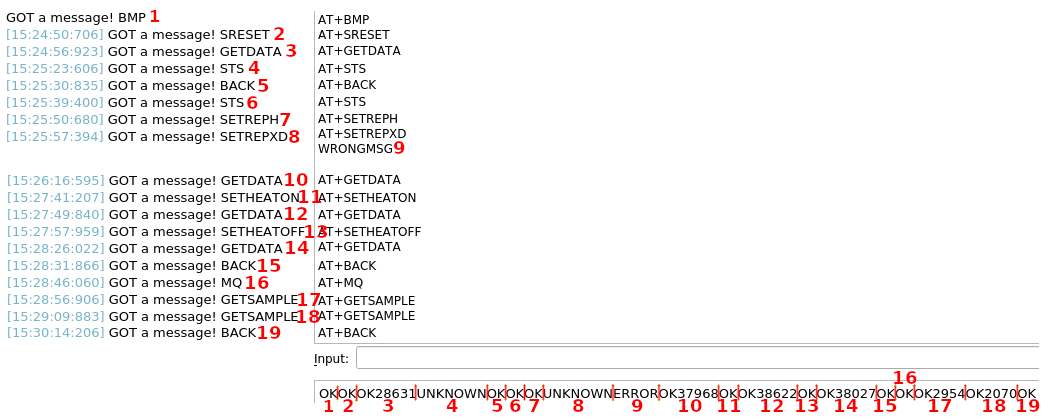
\includegraphics[width=\textwidth, height=\textheight, keepaspectratio]{Graphics/logs.png}
    \caption{Zapis programu cutecom. Po lewej konsola DEBUG, po prawej komendy wysyłane do mikroprocesora, na dole odpowiedzi na kolejne komendy}
    \label{img:cutecom}
\end{figure}

Dodatkową funkcjonalnością którą należało przetestować, było ustawianie konfiguracji czujników przy użyciu parametrów przekazywanych do mikroprocesora. Na obrazku \ref{img:args} widać, że czujnik BMP280 poprawnie przyjmuje konfigurację, gdy zawiera ona cztery parametry (zwraca bajty \textit{,,OK0''}). Po ustawieniu nowej konfiguracji, poprawnie zwraca wartości ciśnienia i temperatury (\textit{,,OK[value]''}). Po przesłaniu niepoprawnej komendy \textit{AT+SETCONFIG,96,20,0,1,7,7,7,7,7} zawierającej zbyt dużą ilość argumentów, układ zgodnie z oczekiwaniami zwrócił bajty \textit{,,OK1''}. \textit{OK} oznacza tutaj poprawne rozpoznanie komendy, natomiast \textit{1} niepowodzenie w jej wykonaniu. W tym miejscu można wskazać kolejne miejsce na rozbudowę oprogramowania. Opisywane wcześniej ustandaryzowane w obrębie programu kody błędy, mogłyby być zwracane do użytkownika, informując go o problemie który wystąpił.

\begin{figure}[H]
    \centering
    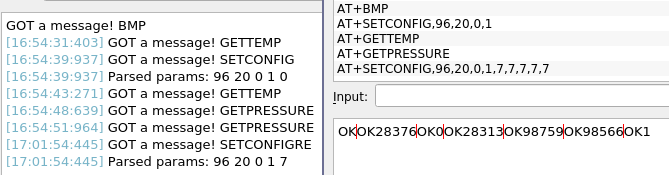
\includegraphics[width=\textwidth, height=\textheight, keepaspectratio]{Graphics/args.png}
    \caption{Zapis programu cutecom. Po lewej konsola DEBUG, po prawej komendy wysyłane do mikroprocesora, na dole odpowiedzi na kolejne komendy}
    \label{img:args}
\end{figure}
\chapter{Wnioski}
\label{cha:results}
W trakcie trwania projektu poruszono zarówno aspekty dotyczące projektowania sprzętu, jak i tworzenia oprogramowania. Sam projekt, na pewno był projektem złożonym i wymagającym. Zaprojektowanie płytki, wymagało czasochłonnej analizy dokumentacji układów, a nawet przypomnienia sobie zagadnień elektroniki analogowej. Mimo to, popełniono wiele błędów opisanych we wcześniejszych rozdziałach. W trakcie tworzenia kolejnej rewizji sprzętu, należałoby więc uwzględnić omówione zmiany. Dodatkowo, elementy pasywne w obudowach 0805, które wydawały się dobrą decyzją pod kątem ręcznego lutowania płytek, okazały się niepotrzebnym utrudnieniem. W kolejnej rewizji, należałoby zastosować elementy w obudowach 0603. Dzięki temu, oszczędzonoby wiele miejsca, co pozwoliłoby na efektywniejsze wykorzystanie dostępnej powierzchnii. Kolejnym istotnym wnioskiem, jest sam dobór czujników na płytce. W przypadku tego projektu, głównym założeniem było przetestowanie różnych interfejsów na płytce z mikroprocesorem. W przypadku płytki komercyjnej, zastosowanie czujnika z grzałką obok czujnika temperatury, byłoby zupełnie pozbawione sensu. Wyjątkiem, byłoby dodanie układu sterującego zasilaniem czujnika z grzałką. Cennym wnioskiem wydaje się być również fakt, że błędy w przypadku projektowania sprzętu, są nieuniknione i w przypadku chęci stworzenia produktu, na etapie planowania należy uwzględnić wykonanie kilku kolejnych rewizji sprzętu. W przypadku tego projektu, mimo sprawdzania layoutu oraz schematu przez kilka osób z doświadczeniem, błędy i tak się pojawiły. W przypadku tworzenia oprogramowania, najważniejszym z wniosków wydaje się być fakt, że należy wzajemnie sprawdzać kod w obrębie zespołu. Pozwala to nie tylko wychwycić wiele błędów, ale przede wszystkim nauczyć się zupełnie nowych sposobów tworzenia kodu. Błędem, była natomiast próba stworzenia oprogramowania działającego na dwóch zupełnie różnych mikroprocesorach. Decyzja o takim podejściu podyktowana była założeniem, że HAL dostarczony przez ST, rozwiązuje kwestie kompatybilności między układami. Tymczasem okazało się, że wyjątkowo dużo czasu zostało zmarnowane na próby uruchomienia kodu stworzonego na innej płytki. Pojawiające się rozbieżności w nazwach stałych z bibliotek ST, różne sposoby konfiguracji peryferiów oraz potrzeba korzystania z różnych bibliotek sprawiła, że część kodu była tak na prawdę pisana dwa razy.\newline
W tym wszystkim należy zaznaczyć, że stworzony projekt znacząco przekraczał podstawowe założenia przedmiotu, jednak od początku jego celem była chęć praktycznego sprawdzania omawianych zagadnień. Można więc powiedzieć, że jego wykonanie było sztuką dla sztuki. Dzięki temu, pozwolił on nie tylko na zdobycie nowych umiejętności, ale również przyjemne spędzenie czasu.


\printbibliography

\end{document}